\documentclass[11pt]{article}

\usepackage{centernot}
\usepackage{amssymb}
\usepackage{xcolor}
\usepackage{verbatim}
\usepackage{multicol}
\usepackage{enumitem}
\usepackage{amsfonts}
\usepackage{amsmath}
\usepackage[utf8]{inputenc}
\usepackage[export]{adjustbox}  % for correct logo rendering
\usepackage{fancyhdr}  % for header/footer formatting
\usepackage{hyperref}  % for hyper-references
\usepackage{datetime}  % to update month in footer
\usepackage{array}  % more flexible tables
\usepackage[includeheadfoot,
            left=1in,
            right=1in,
            top=0.75in,
            bottom=0.75in,
            headheight=40pt]{geometry} % geometry needs to know headheight to correctly render the footer
\usepackage{tikz} % For drawing grid boxes

\definecolor{darkblue}{RGB}{0, 0, 139}
\definecolor{lightblue}{RGB}{173, 216, 230}

% desired format for footer
\newdateformat{monthyeardate}{%
  \monthname[\THEMONTH] \THEYEAR}

% set up header/footer
\pagestyle{fancy}
\fancyhf{}  % clear all headers/footers
\renewcommand{\headrulewidth}{0pt}  % remove header rule
\renewcommand{\footrulewidth}{0pt}  % remove footer rule

% set up header

\fancypagestyle{firstpage}{
    \fancyhead[L]{
    \vspace{0pt}
    \hspace{-8pt}
    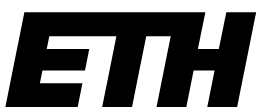
\includegraphics[width=0.1\textwidth]{docimgs/eth_logo_kurz_pos.png}\\
    \textbf{Swiss Federal Institute of Technology}\\
    \textbf{Zurich}\\
    %\textbf{ } \\
    
    }    

    \fancyhead[R]{
    \raggedleft
    %\vspace{20pt}
    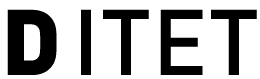
\includegraphics[width=0.13\textwidth]{docimgs/eth_ditet_logo_pos.png}\\
     \textbf{Dept. of Information Technology and} \\ \textbf{Electrical Engineering}  \\
     %\textbf{Chair for Mathematical Information} \\ \textbf{Information Science} \\

    }
}

% set up footer
\fancyfoot[L]{mdietz, ÜS 5}
\fancyfoot[C]{\thepage}
\fancyfoot[R]{\monthyeardate\today}

% set up section/subsection titles
\renewcommand{\thesection}{\arabic{section}}
\renewcommand{\thesubsection}{\arabic{subsection}}

% command used for simply emphasizing suggestions
\newcommand{\suggestion}[1]{{\itshape #1}}

%--- commands for transform arrows----------------
\newcommand{\transform}[2]{%
    \begin{tikzpicture}
        % Open circle
        \draw[thick] (0,0) circle (0.1);
        % Line with number above and adjustable length
        \draw[thick] (0.1,0) -- (#2,0) node[midway, above] {#1};
        % Filled circle
        \filldraw[thick] (#2,0) circle (0.1);
    \end{tikzpicture}%
}
\newcommand{\invtransform}[2]{%
    \begin{tikzpicture}
        % filled circle
        \filldraw[thick] (0,0) circle (0.1);
        % Line with number above and adjustable length
        \draw[thick] (0.1,0) -- (#2 -0.1,0) node[midway, above] {#1};
        % open circle
        \draw[thick] (#2,0) circle (0.1);
    \end{tikzpicture}%
}
\newcommand{\verticaltransform}[4]{%
    \begin{tikzpicture}
        % Open circle at the bottom with text below
        \filldraw[thick] (0,0) circle (0.1) node[below=3pt] {$#4$};
        % Vertical line with number on the left
        \draw[thick] (0,0.1) -- (0,#2 -0.1) node[midway, left] {#1};
        % Filled circle at the top with text above
        \draw[thick] (0,#2) circle (0.1) node[above=3pt] {$#3$};
    \end{tikzpicture}%
}
\newcommand{\verticalinvtransform}[4]{%
    \begin{tikzpicture}
        % Open circle at the bottom with text below
        \draw[thick] (0,0) circle (0.1) node[below=3pt] {$#4$};
        % Vertical line with number on the left
        \draw[thick] (0,0.1) -- (0,#2) node[midway, left] {#1};
        % Filled circle at the top with text above
        \filldraw[thick] (0,#2) circle (0.1) node[above=3pt] {$#3$};
    \end{tikzpicture}%
}

\begin{document}
\thispagestyle{firstpage}

\setlength{\headheight}{1 \baselineskip}  % accomodate header
\setlength{\parindent}{0pt}  % remove initial paragraph indent
\setlength{\parskip}{\baselineskip}  % add skip between paragraphs

\vspace*{-5px}
\section*{Übungsstunde 5}

\section*{Themenüberblick}
\begin{itemize}
    \item \textbf{Verallgemeinerte Funktionen:}
    \item[] Funktionale
    \item[] $\delta-$Funktion und ihre Eigenschaften
    \item[] Ableitung verallgemeinerter Funktionen
\end{itemize}

\section*{Aufgaben für diese Woche}
\vspace{-0.5cm}

\underline{\textbf{46}}, 47, \underline{\textbf{48}}, \underline{\textbf{49}}, \underline{\textbf{50}}, \underline{\textbf{51}}, 52, 53, \underline{\textbf{54}}, \underline{\textbf{55}}\\
\vspace{-0.5cm}

Die \underline{\textbf{fettgedruckten}} Übungen empfehle ich, weil sie wesentlich zu eurem Verständnis der Theorie beitragen und/oder sehr prüfungsrelevant sind.

\vfill \null
\pagebreak

\section*{Verallgemeinerte Funktionen}
\vspace*{-0.5cm}
Dieses Kapitel ist nicht wirklich prüfungsrelevant. Es dient mehr zur theoretischen Herleitung und eurem Verständnis der Deltafunktion.
\vspace*{-0.5cm}
\subsection*{Funktional}
\vspace*{-0.5cm}
Ein Funktional ist eine Funktion, deren Definitionsmenge eine Teilmenge eines linearen Raumes $X$ ist und deren Zielmenge aus Skalaren besteht.

\textbf{Mittelwertsatz} der Integration: $\exists \xi \in [a,b], \; \text{  sodass  } \; \ell_x(\varphi) = \displaystyle\int_a^b \varphi(t)x(t)dt = x(\xi)\displaystyle\int_a^b \varphi(t)dt$
\vspace*{-0.5cm}
\begin{center}
    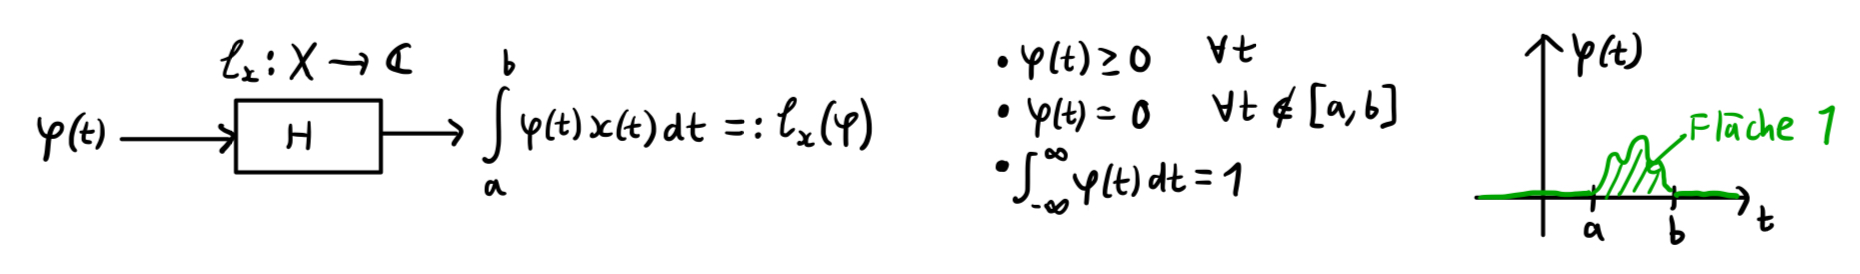
\includegraphics[width=\linewidth]{docimgs/Funktionale_1.jpg}
\end{center}

\vspace*{-0.5cm}
\subsection*{Herkömmlicher Funktionenbegriff als Spezialfall}
\vspace*{-0.5cm}
\subsubsection*{Deltafolge}
\vspace*{-0.5cm}
Eine Deltafolge $\delta_n(t)$ hat folgende Eigenschaften:
\vspace*{-0.5cm}
\begin{enumerate}
    \item $\delta_n(t) \begin{cases}
        \geq 0, \hspace{20pt} \forall t \in I_n = [a_n, b_n]\\
        = 0, \hspace{20pt} \forall t \notin I_n
    \end{cases}$
    \item Die Intervalle $I_n$ bilden eine Intervallverschachtelung für $t_0 \in \mathbb{R}$, d.h. die Intervalle, auf denen $\delta_n(t) \geq 0$ werden immer schmäler: $a_1 \leq a_2 \leq \dots \leq t_0 \leq \dots \leq b_2 \leq b_1$
    \item[] und $\displaystyle\lim_{n \to \infty}a_n = \displaystyle\lim_{n \to \infty}b_n = t_0$
    \item Normierung: $\forall n$ gilt $\displaystyle\int_{-\infty}^\infty \delta_n(t)\text{d}t = \displaystyle\int_{a_n}^{b_n}\delta_n(t)\text{d}t = 1$
    \item[] Graphisch sehen Punkte 1.-3. wie folgt aus:
\end{enumerate}
\begin{center}
    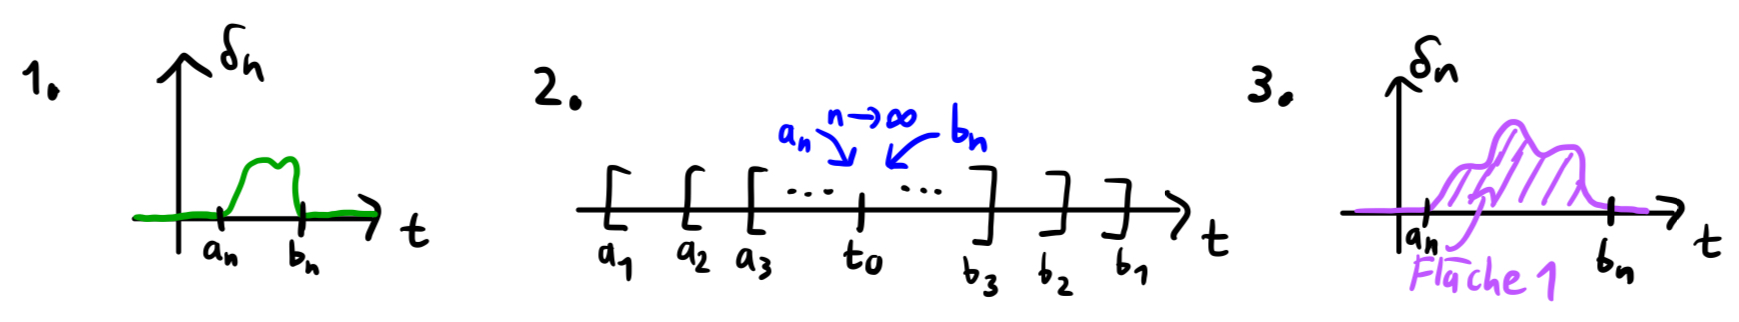
\includegraphics[width=0.9\linewidth]{docimgs/Deltafolge_1.jpg}
\end{center}

\vfill \null
\pagebreak

Eine mögliche Deltafolge wäre zum Beispiel:
\begin{center}
    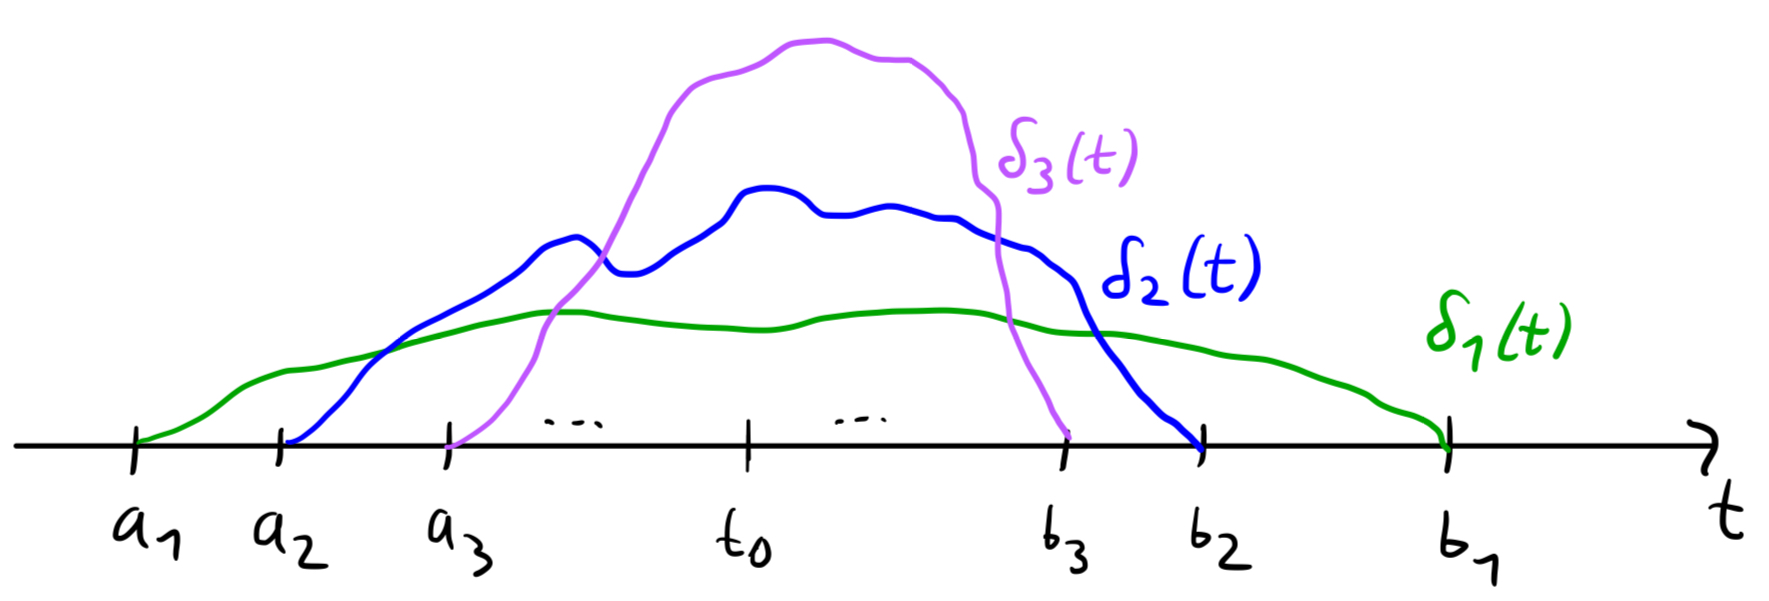
\includegraphics[width=0.6\linewidth]{docimgs/Deltafolge_2.jpg}
\end{center}
Wir nehmen nun den Grenzwert für $n \to \infty$ und erhalten die \textbf{Dirac-Delta} "Funktion":
$$\delta_{t_0}(t) := \lim_{n \to \infty} \delta_n(t) \; \begin{cases}
    \to \infty, \hspace{20pt} t = t_0\\
    = 0, \hspace{28pt} t \neq t_0
\end{cases} = \delta(t-t_0)$$
Die Dirac-Delta Funktion ist im herkömmlichen Sinn keine echte Funktion. Ihre Eigenschaften sind, dass sie Breite $0$, Höhe $\to \infty$ und Fläche $1$ hat.

\subsection*{Die Deltafunktion}
\vspace*{-0.5cm}
Wir betrachten die Funktion:
$$\delta(t, \varepsilon) = \begin{cases}
        \frac{1}{2\varepsilon} \hspace{12pt} |t|\leq \varepsilon\\
        0, \hspace{20pt} \text{sonst}
    \end{cases}$$
\begin{itemize}[leftmargin = 0pt]
    \item[] Dann $\ell_x(\delta(t, \varepsilon)) = \displaystyle\int_{-\infty}^{\infty} x(t) \delta(t, \varepsilon)\text{d}t = x(\xi) \displaystyle\int_{-\varepsilon}^\varepsilon \delta(t, \varepsilon)\text{d}t = x(\xi)$
    \item[] Wir lassen $\varepsilon \to 0$, dann $\xi \to 0$ und somit $\displaystyle\lim_{\varepsilon \to 0} \ell_x(\delta(t, \varepsilon)) = x(0)$. Man schreibt $\delta(t) = \displaystyle\lim_{\varepsilon \to 0}\delta(t,\varepsilon)$
\end{itemize}
\begin{center}
    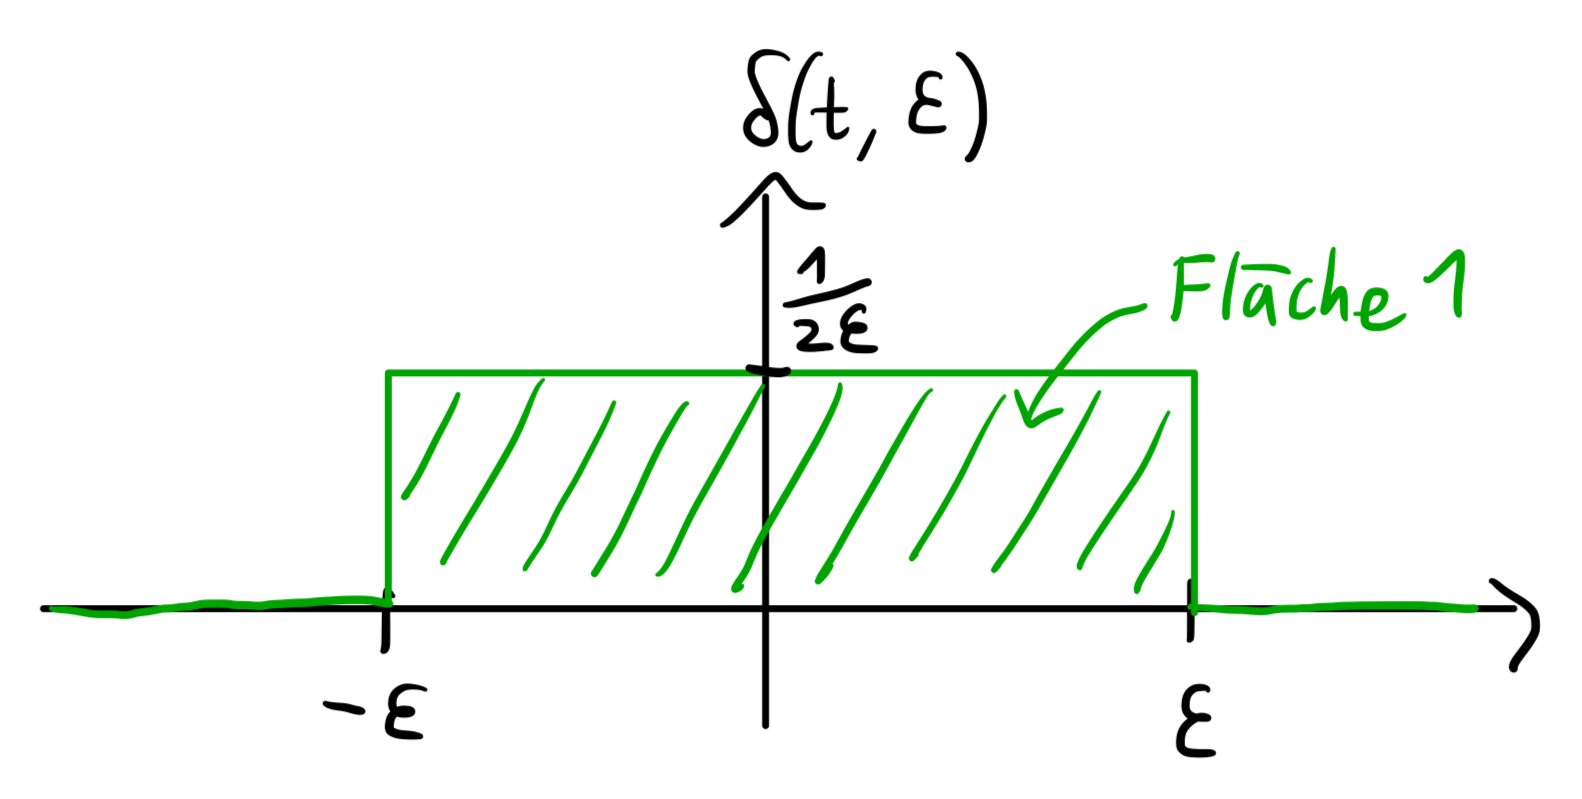
\includegraphics[width=0.4\linewidth]{docimgs/Deltafunktion_1.jpg}
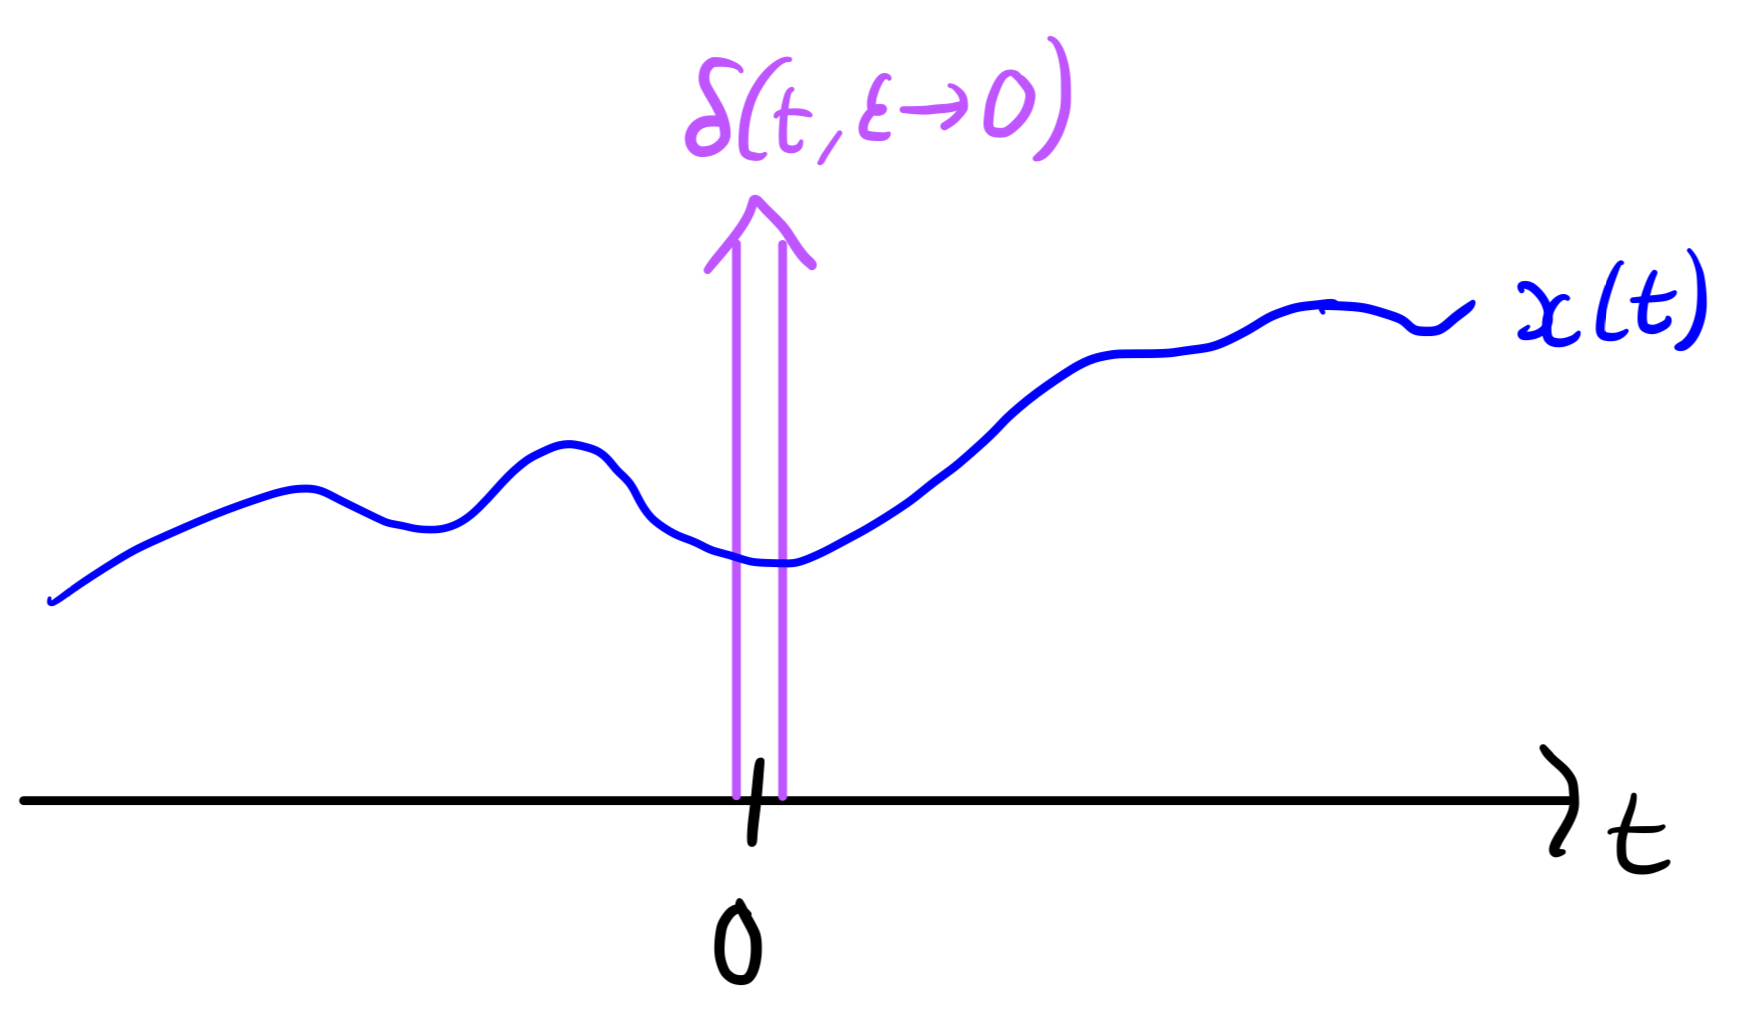
\includegraphics[width=0.4\linewidth]{docimgs/Deltafunktion_2.jpg}
\end{center}
$$\implies \delta(t)x(t) = \delta(t)x(0), \hspace{12pt} \text{ dann } \hspace{12pt} \int_{-\infty}^{\infty} x(t)\delta(t) \text{d}t = \int_{-\infty}^{\infty} x(0)\delta(t) \text{d}t = x(0)\int_{-\infty}^{\infty}\delta(t) \text{d}t = x(0)$$

\vfill \null
\pagebreak

\section*{Eigenschaften der $\delta-$Funktion}
\vspace*{-0.5cm}
Die folgenden Eigenschaften sind sehr wichtig für die Aufgaben in SST1. Am wichtigsten sind die \textbf{3.} und \textbf{5.} Eigenschaft. Diese muss man in jeder Prüfung mehrfach anwenden.
\vspace*{-0.5cm}
\begin{enumerate}
    \item \textbf{Symmetrie}: 
    \item[] $\delta(t) = \delta(-t)$
    \item[] $\delta(t-t_0) = \delta(t_0 - t)$
    \item \textbf{Multiplikation mit einer Funktion}: \item[] $x(t)\delta(t) = x(0)\delta(t)$
    \item[] $x(t)\delta(t-t_0)=x(t_0)\delta(t-t_0)$
    \item \textbf{Siebeigenschaft}: 
    \item[] $\displaystyle\int_{-\infty}^{\infty}\delta(t)x(t)\text{d}t = x(0)$
    \item[] $\displaystyle\int_{-\infty}^{\infty}\delta(t-t_0)x(t)\text{d}t = x(t_0)$
    \item \textbf{Verschiebung/Skalierung des Parameters}:
    \item[] $\delta(at + b) = \displaystyle\frac{1}{|a|}\delta\left(t + \displaystyle\frac{b}{a} \right)$
    \item \textbf{Die $\delta-$Funktion ist das Einselement der Faltung}:
    \item[] $(x \ast \delta)(t) = \displaystyle\int_{-\infty}^\infty x(t-\tau)\delta(\tau)\text{d}\tau = x(t)$
    \item[] $(x \ast \delta(\cdot - t_0))(t) = x(t - t_0)$
    \item \textbf{Einheitssprungfunktion}:
    \item[] $\displaystyle\int_{-\infty}^t \delta(\tau) \text{d}\tau = \sigma(t)$
\end{enumerate}

\vspace*{-0.5cm}
\subsection*{Ableitung von verallgemeinerten Funktionen}
\vspace*{-0.5cm}
Mit $D$ bezeichnen wir den Ableitungsoperator, $x'(t)$ beschreibt die konventionelle Definition der Ableitung einer stetigen, differenzierbaren Funktion, wie wir es aus Analysis 1 kennen, und $t_0$ ist eine Sprungstelle von $x(t)$.
$$(Dx)(t) = x'(t) + (x(t_0^+)- x(t_0^-))\delta(t-t_0)$$

\vfill \null
\pagebreak

\subsubsection*{Bemerkung}
\vspace*{-0.5cm}
Die Impulsantwort ist definiert als $h(t) = (H \delta)(t)$ und die Sprungantwort als $a(t) = (H\sigma)(t)$.\\
\fcolorbox{darkblue}{lightblue}{%
\parbox{\dimexpr\linewidth-2\fboxsep-2\fboxrule\relax}{
    \begin{center}
        Da $\displaystyle\frac{\text{d}\sigma(t)}{\text{d}t} = \delta(t)$ haben wir $\displaystyle\frac{\text{d}a(t)}{\text{d}t} = h(t)$
    \end{center}
}}%

\subsection*{Aufgabe 50}
\vspace*{-0.5cm}
Welche der folgenden verallgemeinerten Funktionen sind identisch?
\begin{multicols}{2}
\begin{itemize}
    \item[a)] $2t^2 \delta(t-1)$
    \item[b)] $(t+2)\delta(t-1)$
    \item[c)] $2e^{t-1}\delta(1-t)$
    \item[d)] $(t+2)^2 \delta(3t-3)$
\end{itemize}
\end{multicols}
\vspace*{-0.5cm}

\begin{tikzpicture}
    % Define the box size and grid spacing
    \draw[step=0.5cm,gray!50,very thin] (0,0) grid (16.5,3
    ); % (0,0) is bottom-left corner, (10,10) is top-right corner
\end{tikzpicture}

\vspace*{-0.5cm}
\subsection*{Aufgabe 51}
\vspace*{-0.5cm}
Berechnen Sie die Ableitungen der folgenden Signale bzw. verallgemeinerter Funkionen:
\vspace*{-0.5cm}
\begin{itemize}
    \item[a)] $x(t) = |t|$
    \item[c)]
    \item[] \vspace{-0.75cm}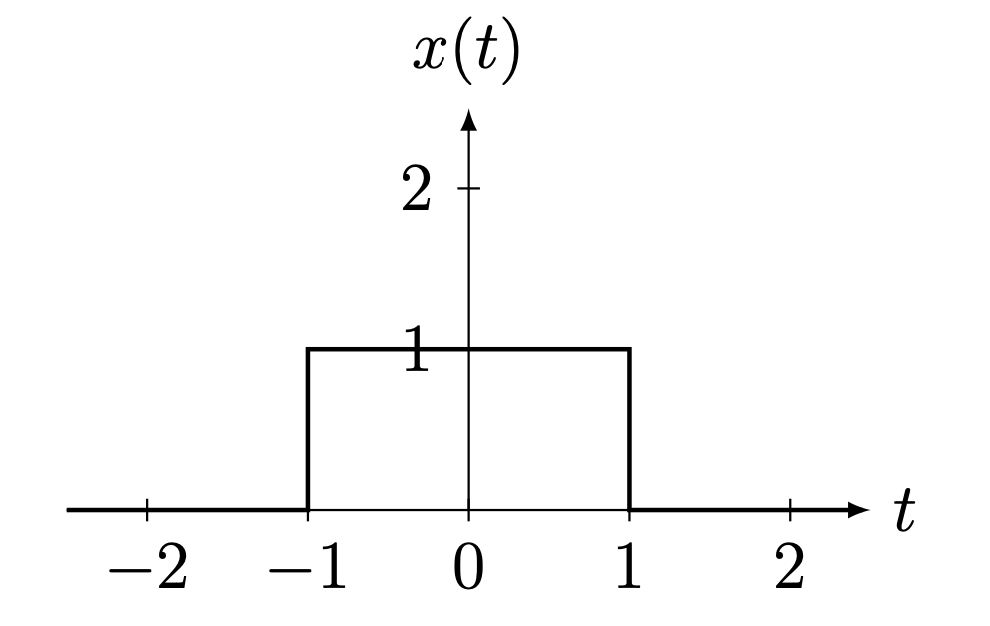
\includegraphics[width=0.3\linewidth]{docimgs/51c).png}
\end{itemize}


\begin{tikzpicture}
    % Define the box size and grid spacing
    \draw[step=0.5cm,gray!50,very thin] (0,0) grid (16.5,4
    ); % (0,0) is bottom-left corner, (10,10) is top-right corner
\end{tikzpicture}

\end{document}
